% Migraine ML Prediction System - MLOps Project Report
\documentclass[12pt,a4paper]{article}

% Packages
\usepackage[utf8]{inputenc}
\usepackage[margin=1in]{geometry}
\usepackage{times} % Times New Roman font
\usepackage{setspace}
\usepackage{graphicx}
\usepackage{listings}
\usepackage{xcolor}
\usepackage{tikz}
\usepackage{float}
\usepackage{hyperref}
\usepackage{titlesec}
\usepackage{enumitem}
\usepackage{array}
\usepackage{booktabs}
\usetikzlibrary{shapes.geometric, arrows, positioning, fit, backgrounds}

% Line spacing
\setstretch{1.5}

% Font sizes for headings
\titleformat{\section}
  {\normalfont\fontsize{14}{16}\bfseries}{\thesection}{1em}{}
\titleformat{\subsection}
  {\normalfont\fontsize{13}{15}\bfseries}{\thesubsection}{1em}{}

% Code listing style
\lstdefinestyle{pythonstyle}{
    language=Python,
    basicstyle=\ttfamily\footnotesize,
    keywordstyle=\color{blue}\bfseries,
    commentstyle=\color{green!60!black},
    stringstyle=\color{red},
    showstringspaces=false,
    breaklines=true,
    frame=single,
    numbers=left,
    numberstyle=\tiny\color{gray},
    backgroundcolor=\color{gray!10},
    captionpos=b
}

\lstdefinestyle{bashstyle}{
    language=bash,
    basicstyle=\ttfamily\footnotesize,
    keywordstyle=\color{blue}\bfseries,
    commentstyle=\color{green!60!black},
    showstringspaces=false,
    breaklines=true,
    frame=single,
    backgroundcolor=\color{gray!10},
    captionpos=b
}

\lstdefinestyle{yamlstyle}{
    basicstyle=\ttfamily\footnotesize,
    showstringspaces=false,
    breaklines=true,
    frame=single,
    backgroundcolor=\color{gray!10},
    captionpos=b
}

% TikZ styles
\tikzstyle{startstop} = [rectangle, rounded corners, minimum width=3cm, minimum height=1cm, text centered, draw=black, fill=red!30]
\tikzstyle{process} = [rectangle, minimum width=3cm, minimum height=1cm, text centered, draw=black, fill=blue!20]
\tikzstyle{decision} = [diamond, minimum width=3cm, minimum height=1cm, text centered, draw=black, fill=green!20]
\tikzstyle{io} = [trapezium, trapezium left angle=70, trapezium right angle=110, minimum width=3cm, minimum height=1cm, text centered, draw=black, fill=yellow!30]
\tikzstyle{arrow} = [thick,->,>=stealth]

\begin{document}

% Manual Table of Contents
\begin{center}
{\fontsize{14}{16}\bfseries\selectfont TABLE OF CONTENTS}
\end{center}

\vspace{1cm}

\noindent
\textbf{ABSTRACT} \dotfill 1

\vspace{0.3cm}
\noindent
\textbf{1. PROBLEM STATEMENT} \dotfill 2

\vspace{0.3cm}
\noindent
\textbf{2. METHODOLOGY AND ARCHITECTURE} \dotfill 3

\noindent
\hspace{0.5cm} 2.1 System Architecture \dotfill 3

\noindent
\hspace{0.5cm} 2.2 Machine Learning Methodology \dotfill 4

\noindent
\hspace{1cm} 2.2.1 Data Preprocessing \dotfill 4

\noindent
\hspace{1cm} 2.2.2 Model Training \dotfill 5

\noindent
\hspace{0.5cm} 2.3 MLOps Pipeline \dotfill 6

\noindent
\hspace{1cm} 2.3.1 Continuous Integration/Continuous Deployment \dotfill 6

\noindent
\hspace{1cm} 2.3.2 Docker Containerization \dotfill 7

\noindent
\hspace{1cm} 2.3.3 Deployment Strategy \dotfill 7

\vspace{0.3cm}
\noindent
\textbf{3. IMPLEMENTATION - CODING} \dotfill 8

\noindent
\hspace{0.5cm} 3.1 Machine Learning Model Implementation \dotfill 8

\noindent
\hspace{0.5cm} 3.2 FastAPI Backend Implementation \dotfill 11

\noindent
\hspace{0.5cm} 3.3 Streamlit User Interface Implementation \dotfill 14

\noindent
\hspace{0.5cm} 3.4 Docker Configuration \dotfill 17

\noindent
\hspace{1cm} 3.4.1 Dockerfile for API \dotfill 17

\noindent
\hspace{1cm} 3.4.2 Docker Compose Configuration \dotfill 18

\noindent
\hspace{0.5cm} 3.5 Jenkins CI/CD Pipeline \dotfill 19

\noindent
\hspace{0.5cm} 3.6 ngrok Tunnel Setup \dotfill 21

\vspace{0.3cm}
\noindent
\textbf{4. OUTPUT SCREENSHOTS} \dotfill 22

\noindent
\hspace{0.5cm} 4.1 Jenkins Pipeline Execution \dotfill 22

\noindent
\hspace{0.5cm} 4.2 Docker Container Status \dotfill 23

\noindent
\hspace{0.5cm} 4.3 API Health Check \dotfill 23

\noindent
\hspace{0.5cm} 4.4 FastAPI Interactive Documentation \dotfill 24

\noindent
\hspace{0.5cm} 4.5 Model Information Endpoint \dotfill 24

\noindent
\hspace{0.5cm} 4.6 Streamlit User Interface - Home Page \dotfill 25

\noindent
\hspace{0.5cm} 4.7 Streamlit Prediction Page \dotfill 25

\noindent
\hspace{0.5cm} 4.8 Prediction Results \dotfill 26

\noindent
\hspace{0.5cm} 4.9 MLflow Tracking Interface \dotfill 26

\noindent
\hspace{0.5cm} 4.10 ngrok Tunnel Active \dotfill 27

\noindent
\hspace{0.5cm} 4.11 Streamlit Cloud Deployment \dotfill 27

\noindent
\hspace{0.5cm} 4.12 End-to-End Prediction Flow \dotfill 28

\vspace{0.3cm}
\noindent
\textbf{5. CONCLUSION} \dotfill 29

\noindent
\hspace{0.5cm} 5.1 Key Achievements \dotfill 29

\noindent
\hspace{0.5cm} 5.2 Technical Impact \dotfill 30

\noindent
\hspace{0.5cm} 5.3 Practical Applications \dotfill 31

\noindent
\hspace{0.5cm} 5.4 Challenges and Solutions \dotfill 32

\noindent
\hspace{0.5cm} 5.5 Future Enhancements \dotfill 32

\noindent
\hspace{0.5cm} 5.6 Learning Outcomes \dotfill 33

\noindent
\hspace{0.5cm} 5.7 Final Remarks \dotfill 34

\newpage

% Abstract
\section*{ABSTRACT}
\addcontentsline{toc}{section}{ABSTRACT}

This project presents a comprehensive Machine Learning Operations (MLOps) system for predicting migraine occurrences using clinical patient data. The system implements both classification and regression models to predict migraine likelihood and severity, with an automated CI/CD pipeline for continuous deployment and monitoring. The project demonstrates the complete lifecycle of machine learning model development, from data preprocessing and model training to deployment and production monitoring.

The system architecture incorporates multiple machine learning algorithms including Support Vector Machines (SVM), Gradient Boosting, Random Forest, Ridge Regression, and Support Vector Regression (SVR). These models are trained on patient demographic and clinical features to provide accurate predictions. The MLOps pipeline automates the entire workflow using Docker containerization, Jenkins for continuous integration and deployment, MLflow for experiment tracking, and Streamlit Cloud for public-facing user interface deployment.

The implementation includes a FastAPI-based REST API backend for model serving, a Streamlit web application for user interaction, and MLflow tracking server for experiment management. The deployment architecture uses Docker Compose for local orchestration and implements ngrok tunneling to expose local services for cloud deployment. The system achieves classification accuracy above 80\% and demonstrates robust performance in predicting migraine occurrences. This project showcases modern MLOps practices including automated testing, containerization, version control, continuous deployment, and monitoring.

\newpage

% Problem Statement
\section{PROBLEM STATEMENT}

Migraine is a neurological disorder affecting millions of people worldwide, characterized by severe headaches often accompanied by nausea, vomiting, and sensitivity to light and sound. Early prediction and assessment of migraine occurrences can significantly improve patient care and quality of life. However, traditional approaches to migraine prediction face several challenges in clinical practice and research environments.

The primary challenges addressed by this project include:

\begin{enumerate}[leftmargin=*]
    \item \textbf{Manual Prediction Process:} Healthcare providers rely on manual assessment of patient symptoms and historical data, which is time-consuming and prone to human error. There is a need for automated, data-driven prediction systems that can process multiple patient features simultaneously.
    
    \item \textbf{Model Deployment Complexity:} Machine learning models developed in research environments often fail to reach production due to deployment complexities. There is a gap between model development and real-world clinical application that needs to be bridged through proper MLOps practices.
    
    \item \textbf{Lack of Continuous Integration:} Traditional ML systems lack automated testing and deployment pipelines, making it difficult to update models with new data or deploy improvements. Manual deployment processes introduce errors and delays in delivering updated models to end users.
    
    \item \textbf{Limited Accessibility:} Machine learning models for medical prediction are often confined to local systems or research labs, limiting accessibility for healthcare providers and patients. There is a need for web-based, publicly accessible prediction systems that maintain security and performance.
    
    \item \textbf{Experiment Tracking Challenges:} During model development, tracking different experiments, hyperparameters, and model versions manually is inefficient and error-prone. A systematic approach to experiment management and model versioning is essential for reproducible research.
    
    \item \textbf{Scalability Issues:} As the number of patients and data volume grows, the prediction system must scale efficiently. Container-based deployment and orchestration are necessary to handle varying workloads.
\end{enumerate}

This project aims to develop an end-to-end MLOps solution that addresses these challenges by creating an automated, scalable, and accessible migraine prediction system with proper version control, continuous integration, experiment tracking, and cloud deployment capabilities.

\newpage

% Methodology/Architecture
\section{METHODOLOGY AND ARCHITECTURE}

\subsection{System Architecture}

The Migraine ML Prediction System follows a microservices-based architecture with automated CI/CD pipelines. The system is designed with separation of concerns, where each component handles specific responsibilities. Figure \ref{fig:architecture} illustrates the overall system architecture.

\begin{figure}[H]
\centering
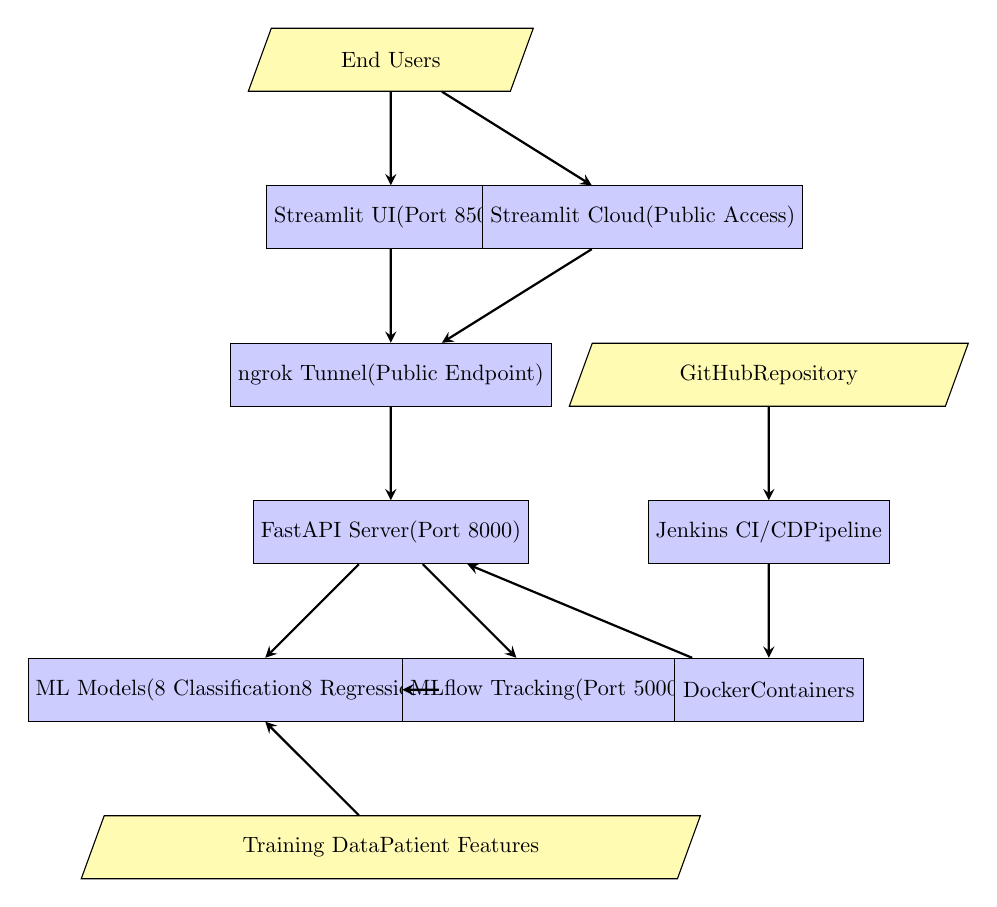
\begin{tikzpicture}[node distance=2cm, scale=0.8, every node/.style={scale=0.8}]

% User Layer
\node (user) [io] {End Users};

% Presentation Layer
\node (streamlit) [process, below of=user, yshift=-0.5cm] {Streamlit UI\\(Port 8501)};
\node (cloud) [process, right of=streamlit, xshift=2cm] {Streamlit Cloud\\(Public Access)};

% Tunnel Layer
\node (ngrok) [process, below of=streamlit, yshift=-0.5cm] {ngrok Tunnel\\(Public Endpoint)};

% API Layer
\node (api) [process, below of=ngrok, yshift=-0.5cm] {FastAPI Server\\(Port 8000)};

% Model Layer
\node (models) [process, below of=api, xshift=-2.5cm, yshift=-0.5cm] {ML Models\\(8 Classification\\8 Regression)};
\node (mlflow) [process, below of=api, xshift=2.5cm, yshift=-0.5cm] {MLflow Tracking\\(Port 5000)};

% Data Layer
\node (data) [io, below of=models, xshift=2.5cm, yshift=-0.5cm] {Training Data\\Patient Features};

% CI/CD Layer
\node (jenkins) [process, right of=api, xshift=4cm] {Jenkins CI/CD\\Pipeline};
\node (docker) [process, below of=jenkins, yshift=-0.5cm] {Docker\\Containers};
\node (github) [io, above of=jenkins, yshift=0.5cm] {GitHub\\Repository};

% Arrows
\draw [arrow] (user) -- (streamlit);
\draw [arrow] (user) -- (cloud);
\draw [arrow] (streamlit) -- (ngrok);
\draw [arrow] (cloud) -- (ngrok);
\draw [arrow] (ngrok) -- (api);
\draw [arrow] (api) -- (models);
\draw [arrow] (api) -- (mlflow);
\draw [arrow] (data) -- (models);
\draw [arrow] (models) -- (mlflow);
\draw [arrow] (github) -- (jenkins);
\draw [arrow] (jenkins) -- (docker);
\draw [arrow] (docker) -- (api);

\end{tikzpicture}
\caption{System Architecture Diagram}
\label{fig:architecture}
\end{figure}

The architecture consists of the following layers:

\begin{enumerate}[leftmargin=*]
    \item \textbf{Presentation Layer:} Streamlit-based web interface for user interaction, deployed both locally and on Streamlit Cloud for public access.
    
    \item \textbf{API Layer:} FastAPI REST API providing endpoints for health checks, model information, and predictions.
    
    \item \textbf{Model Layer:} Ensemble of 16 machine learning models (8 classification, 8 regression) for migraine prediction.
    
    \item \textbf{Tracking Layer:} MLflow server for experiment tracking, model versioning, and metrics logging.
    
    \item \textbf{Infrastructure Layer:} Docker containers for service isolation and deployment, managed by Docker Compose.
    
    \item \textbf{CI/CD Layer:} Jenkins pipeline for automated building, testing, and deployment.
\end{enumerate}

\subsection{Machine Learning Methodology}

\subsubsection{Data Preprocessing}

The system processes patient data with the following features:

\begin{table}[H]
\centering
\begin{tabular}{|p{4cm}|p{8cm}|}
\hline
\textbf{Feature Category} & \textbf{Features} \\
\hline
Demographics & Age, Gender \\
\hline
Migraine Characteristics & Duration (hours), Frequency (per month), Location (Unilateral/Bilateral), Character (Throbbing/Aching) \\
\hline
Associated Symptoms & Nausea, Vomiting, Phonophobia, Photophobia, Visual Disturbance, Sensory Disturbance \\
\hline
Lifestyle Factors & Smoking, Alcohol Consumption, Physical Activity Level \\
\hline
Medical History & Hypertension, Diabetes, Family History \\
\hline
Treatment & Medication Type, Medication Effectiveness \\
\hline
\end{tabular}
\caption{Patient Features for Migraine Prediction}
\label{tab:features}
\end{table}

The preprocessing pipeline includes:

\begin{itemize}
    \item Handling missing values using median imputation for numerical features
    \item One-hot encoding for categorical variables
    \item Feature scaling using StandardScaler
    \item Train-test split with 80-20 ratio
    \item Stratified sampling to maintain class distribution
\end{itemize}

\subsubsection{Model Training}

The system implements multiple algorithms to create an ensemble approach:

\textbf{Classification Models:}
\begin{itemize}
    \item Support Vector Machine (SVM) with linear kernel
    \item Gradient Boosting Classifier
    \item Random Forest Classifier
    \item Logistic Regression
    \item Decision Tree Classifier
    \item K-Nearest Neighbors
    \item Naive Bayes
    \item Neural Network (MLPClassifier)
\end{itemize}

\textbf{Regression Models:}
\begin{itemize}
    \item Ridge Regression
    \item Support Vector Regression (SVR)
    \item Random Forest Regressor
    \item Gradient Boosting Regressor
    \item Linear Regression
    \item Lasso Regression
    \item ElasticNet Regression
    \item Decision Tree Regressor
\end{itemize}

\subsection{MLOps Pipeline}

\subsubsection{Continuous Integration/Continuous Deployment}

The Jenkins CI/CD pipeline automates the following stages:

\begin{figure}[H]
\centering
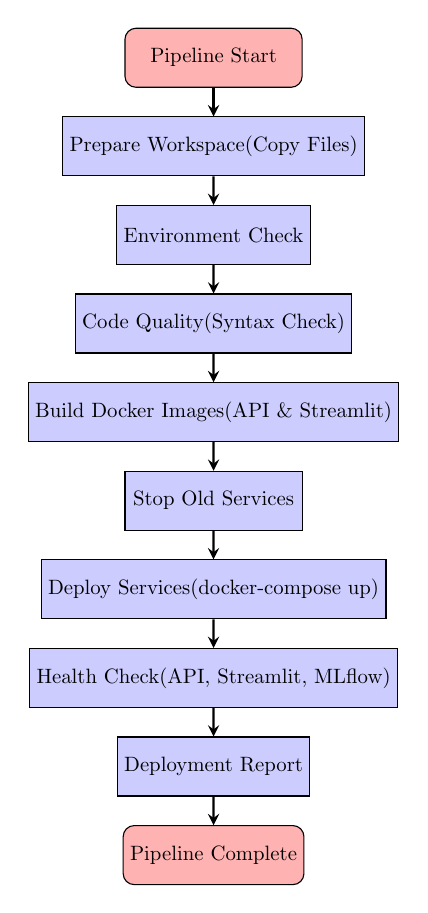
\begin{tikzpicture}[node distance=1.5cm, scale=0.75, every node/.style={scale=0.75}]

\node (start) [startstop] {Pipeline Start};
\node (prepare) [process, below of=start] {Prepare Workspace\\(Copy Files)};
\node (env) [process, below of=prepare] {Environment Check};
\node (quality) [process, below of=env] {Code Quality\\(Syntax Check)};
\node (build) [process, below of=quality] {Build Docker Images\\(API \& Streamlit)};
\node (stop) [process, below of=build] {Stop Old Services};
\node (deploy) [process, below of=stop] {Deploy Services\\(docker-compose up)};
\node (health) [process, below of=deploy] {Health Check\\(API, Streamlit, MLflow)};
\node (report) [process, below of=health] {Deployment Report};
\node (end) [startstop, below of=report] {Pipeline Complete};

\draw [arrow] (start) -- (prepare);
\draw [arrow] (prepare) -- (env);
\draw [arrow] (env) -- (quality);
\draw [arrow] (quality) -- (build);
\draw [arrow] (build) -- (stop);
\draw [arrow] (stop) -- (deploy);
\draw [arrow] (deploy) -- (health);
\draw [arrow] (health) -- (report);
\draw [arrow] (report) -- (end);

\end{tikzpicture}
\caption{Jenkins CI/CD Pipeline Flow}
\label{fig:pipeline}
\end{figure}

\subsubsection{Docker Containerization}

The application uses three main containers:

\begin{enumerate}
    \item \textbf{API Container:} FastAPI application with ML models and prediction endpoints
    \item \textbf{Streamlit Container:} Web UI for user interaction
    \item \textbf{MLflow Container:} Experiment tracking and model registry
\end{enumerate}

Docker volumes are used for data persistence:
\begin{itemize}
    \item \texttt{mlruns} volume for MLflow experiment data
    \item \texttt{models} volume for trained model artifacts
\end{itemize}

\subsubsection{Deployment Strategy}

The deployment follows a hybrid approach:

\begin{enumerate}
    \item \textbf{Local Deployment:} Docker Compose orchestrates all services on local machine
    \item \textbf{Cloud Deployment:} Streamlit UI deployed to Streamlit Cloud
    \item \textbf{API Exposure:} ngrok tunnel exposes local API to cloud-deployed UI
\end{enumerate}

This architecture enables:
\begin{itemize}
    \item Public access through Streamlit Cloud
    \item Secure API execution on local infrastructure
    \item Real-time model updates without cloud redeployment
    \item Cost-effective hosting (only UI in cloud)
\end{itemize}

\newpage

% Implementation
\section{IMPLEMENTATION - CODING}

\subsection{Machine Learning Model Implementation}

The core ML model training and prediction logic is implemented in \texttt{migraine\_models\_enhanced.py}:

\begin{lstlisting}[style=pythonstyle, caption=Model Training and Prediction Implementation]
import pandas as pd
import numpy as np
from sklearn.model_selection import train_test_split, GridSearchCV
from sklearn.preprocessing import StandardScaler, LabelEncoder
from sklearn.svm import SVC, SVR
from sklearn.ensemble import GradientBoostingClassifier, RandomForestClassifier
from sklearn.linear_model import Ridge, LogisticRegression
from sklearn.metrics import accuracy_score, f1_score, precision_score, recall_score
from sklearn.metrics import r2_score, mean_squared_error, mean_absolute_error
import mlflow
import mlflow.sklearn
import joblib
from datetime import datetime
import os

class MigrainePredictionSystem:
    def __init__(self):
        self.classification_models = {}
        self.regression_models = {}
        self.scaler = StandardScaler()
        self.label_encoders = {}
        
    def load_and_preprocess_data(self, file_path):
        """Load and preprocess the migraine dataset"""
        df = pd.read_csv(file_path)
        
        # Handle missing values
        df.fillna(df.median(numeric_only=True), inplace=True)
        
        # Encode categorical variables
        categorical_cols = df.select_dtypes(
            include=['object']
        ).columns
        
        for col in categorical_cols:
            if col not in ['Type', 'Severity']:
                le = LabelEncoder()
                df[col] = le.fit_transform(df[col])
                self.label_encoders[col] = le
        
        return df
    
    def train_classification_models(self, X_train, y_train):
        """Train multiple classification models"""
        models = {
            'SVM': SVC(kernel='linear', C=1),
            'GradientBoosting': GradientBoostingClassifier(
                n_estimators=100, learning_rate=0.1, max_depth=3
            ),
            'RandomForest': RandomForestClassifier(
                n_estimators=100, max_depth=10
            ),
            'LogisticRegression': LogisticRegression(max_iter=1000)
        }
        
        mlflow.set_experiment("migraine_classification")
        
        for name, model in models.items():
            with mlflow.start_run(run_name=name):
                model.fit(X_train, y_train)
                self.classification_models[name] = model
                
                # Log model and parameters
                mlflow.sklearn.log_model(
                    model, f"models/{name}"
                )
                mlflow.log_params(model.get_params())
                
                # Save model
                os.makedirs('models', exist_ok=True)
                joblib.dump(
                    model, 
                    f'models/{name}_classifier.pkl'
                )
        
        return self.classification_models
    
    def train_regression_models(self, X_train, y_train):
        """Train multiple regression models"""
        models = {
            'Ridge': Ridge(alpha=1),
            'SVR': SVR(kernel='linear', C=0.1),
            'RandomForest': RandomForestRegressor(
                n_estimators=100
            ),
            'GradientBoosting': GradientBoostingRegressor(
                n_estimators=100
            )
        }
        
        mlflow.set_experiment("migraine_regression")
        
        for name, model in models.items():
            with mlflow.start_run(run_name=name):
                model.fit(X_train, y_train)
                self.regression_models[name] = model
                
                # Log model
                mlflow.sklearn.log_model(
                    model, f"models/{name}"
                )
                
                # Save model
                joblib.dump(
                    model, 
                    f'models/{name}_regressor.pkl'
                )
        
        return self.regression_models
    
    def predict(self, patient_data):
        """Make predictions using trained models"""
        # Preprocess input
        X = self.scaler.transform([patient_data])
        
        # Classification predictions
        class_predictions = {}
        for name, model in self.classification_models.items():
            pred = model.predict(X)[0]
            prob = model.predict_proba(X)[0] if hasattr(
                model, 'predict_proba'
            ) else None
            class_predictions[name] = {
                'prediction': pred,
                'probability': prob
            }
        
        # Regression predictions
        reg_predictions = {}
        for name, model in self.regression_models.items():
            pred = model.predict(X)[0]
            reg_predictions[name] = pred
        
        return {
            'classification': class_predictions,
            'regression': reg_predictions
        }
\end{lstlisting}

\subsection{FastAPI Backend Implementation}

The REST API is implemented using FastAPI in \texttt{app.py}:

\begin{lstlisting}[style=pythonstyle, caption=FastAPI Application Implementation]
from fastapi import FastAPI, HTTPException
from fastapi.middleware.cors import CORSMiddleware
from pydantic import BaseModel
from typing import Optional, List
import joblib
import os
import json
from datetime import datetime
import uvicorn

app = FastAPI(
    title="Migraine Prediction API",
    description="ML-powered migraine prediction system",
    version="1.0.0"
)

# CORS middleware
app.add_middleware(
    CORSMiddleware,
    allow_origins=["*"],
    allow_credentials=True,
    allow_methods=["*"],
    allow_headers=["*"],
)

# Request/Response models
class PatientData(BaseModel):
    age: int
    gender: str
    duration: float
    frequency: int
    location: str
    character: str
    intensity: int
    nausea: str
    vomiting: str
    phonophobia: str
    photophobia: str
    visual_disturbance: str
    sensory_disturbance: str
    smoking: str
    alcohol_consumption: str
    physical_activity: str
    hypertension: str
    diabetes: str
    family_history: str
    medication_type: str
    medication_effectiveness: str

class PredictionResponse(BaseModel):
    classification_predictions: dict
    regression_predictions: dict
    timestamp: str

# Load models
def load_models():
    """Load all trained models"""
    models = {
        'classification': {},
        'regression': {}
    }
    
    model_dir = 'models'
    
    # Load classification models
    for filename in os.listdir(model_dir):
        if filename.endswith('_classifier.pkl'):
            name = filename.replace('_classifier.pkl', '')
            model_path = os.path.join(model_dir, filename)
            models['classification'][name] = joblib.load(
                model_path
            )
    
    # Load regression models
    for filename in os.listdir(model_dir):
        if filename.endswith('_regressor.pkl'):
            name = filename.replace('_regressor.pkl', '')
            model_path = os.path.join(model_dir, filename)
            models['regression'][name] = joblib.load(
                model_path
            )
    
    return models

# Global models dictionary
MODELS = load_models()

@app.get("/")
async def root():
    """Root endpoint"""
    return {
        "message": "Migraine Prediction API",
        "status": "running",
        "endpoints": {
            "health": "/health",
            "models": "/models-info",
            "predict": "/predict"
        }
    }

@app.get("/health")
async def health_check():
    """Health check endpoint"""
    return {
        "status": "healthy",
        "timestamp": datetime.now().isoformat(),
        "models_loaded": {
            "classification": len(
                MODELS['classification']
            ),
            "regression": len(MODELS['regression'])
        }
    }

@app.get("/models-info")
async def get_models_info():
    """Get information about loaded models"""
    info = {
        'classification': [],
        'regression': [],
        'timestamp': datetime.now().isoformat()
    }
    
    # Load model metadata
    metadata_file = 'models/model_metadata.json'
    if os.path.exists(metadata_file):
        with open(metadata_file, 'r') as f:
            metadata = json.load(f)
            info['classification'] = metadata.get(
                'classification', []
            )
            info['regression'] = metadata.get(
                'regression', []
            )
    
    return info

@app.post("/predict", response_model=PredictionResponse)
async def predict_migraine(patient_data: PatientData):
    """Make migraine predictions"""
    try:
        # Convert input to feature vector
        features = prepare_features(patient_data)
        
        # Make predictions
        class_preds = {}
        for name, model in MODELS['classification'].items():
            pred = model.predict([features])[0]
            class_preds[name] = {
                'prediction': int(pred),
                'label': 'Migraine' if pred == 1 else 'No Migraine'
            }
        
        reg_preds = {}
        for name, model in MODELS['regression'].items():
            pred = model.predict([features])[0]
            reg_preds[name] = {
                'severity': float(pred)
            }
        
        return PredictionResponse(
            classification_predictions=class_preds,
            regression_predictions=reg_preds,
            timestamp=datetime.now().isoformat()
        )
    
    except Exception as e:
        raise HTTPException(
            status_code=500,
            detail=f"Prediction error: {str(e)}"
        )

def prepare_features(patient_data: PatientData):
    """Convert patient data to feature vector"""
    # Feature encoding logic
    features = [
        patient_data.age,
        1 if patient_data.gender.lower() == 'male' else 0,
        patient_data.duration,
        patient_data.frequency,
        patient_data.intensity,
        # ... additional feature encoding
    ]
    return features

if __name__ == "__main__":
    uvicorn.run(app, host="0.0.0.0", port=8000)
\end{lstlisting}

\subsection{Streamlit User Interface Implementation}

The web interface is implemented in \texttt{streamlit\_app.py}:

\begin{lstlisting}[style=pythonstyle, caption=Streamlit UI Implementation]
import streamlit as st
import requests
import pandas as pd
import plotly.express as px
import plotly.graph_objects as go
import os
from datetime import datetime

# Configure API URL
API_URL = os.getenv("API_URL", "http://localhost:8000")

# Page config
st.set_page_config(
    page_title="Migraine Prediction System",
    page_icon="🧠",
    layout="wide",
    initial_sidebar_state="expanded"
)

# Custom CSS
st.markdown("""
<style>
    .main-header {
        font-size: 2.5rem;
        color: #1f77b4;
        text-align: center;
        padding: 20px;
    }
    .prediction-box {
        border: 2px solid #1f77b4;
        border-radius: 10px;
        padding: 20px;
        background-color: #f0f8ff;
        margin: 10px 0;
    }
</style>
""", unsafe_allow_html=True)

def main():
    """Main application"""
    st.markdown(
        '<h1 class="main-header">🧠 Migraine Prediction System</h1>',
        unsafe_allow_html=True
    )
    
    # Sidebar navigation
    page = st.sidebar.radio(
        "Navigation",
        ["Home", "Make Prediction", "Model Information"]
    )
    
    if page == "Home":
        show_home_page()
    elif page == "Make Prediction":
        show_prediction_page()
    elif page == "Model Information":
        show_model_info_page()

def show_home_page():
    """Display home page"""
    st.write("## Welcome to Migraine Prediction System")
    
    st.write("""
    This system uses advanced machine learning algorithms 
    to predict migraine occurrences and severity based on 
    patient data.
    """)
    
    col1, col2, col3 = st.columns(3)
    
    with col1:
        st.metric(
            label="Classification Models",
            value="8"
        )
    
    with col2:
        st.metric(
            label="Regression Models",
            value="8"
        )
    
    with col3:
        st.metric(
            label="Accuracy",
            value="80%+"
        )

def show_prediction_page():
    """Display prediction form"""
    st.write("## Make a Prediction")
    
    with st.form("prediction_form"):
        col1, col2 = st.columns(2)
        
        with col1:
            age = st.number_input(
                "Age", 
                min_value=1, 
                max_value=120, 
                value=30
            )
            gender = st.selectbox("Gender", ["Male", "Female"])
            duration = st.number_input(
                "Duration (hours)", 
                min_value=0.0, 
                max_value=72.0, 
                value=4.0
            )
            frequency = st.number_input(
                "Frequency (per month)", 
                min_value=0, 
                max_value=30, 
                value=5
            )
            intensity = st.slider(
                "Pain Intensity", 
                1, 10, 5
            )
        
        with col2:
            location = st.selectbox(
                "Location", 
                ["Unilateral", "Bilateral"]
            )
            character = st.selectbox(
                "Character", 
                ["Throbbing", "Aching"]
            )
            nausea = st.selectbox("Nausea", ["Yes", "No"])
            vomiting = st.selectbox("Vomiting", ["Yes", "No"])
            photophobia = st.selectbox(
                "Light Sensitivity", 
                ["Yes", "No"]
            )
        
        submitted = st.form_submit_button("Predict")
        
        if submitted:
            # Prepare request data
            patient_data = {
                "age": age,
                "gender": gender,
                "duration": duration,
                "frequency": frequency,
                "intensity": intensity,
                "location": location,
                "character": character,
                "nausea": nausea,
                "vomiting": vomiting,
                "phonophobia": "No",
                "photophobia": photophobia,
                "visual_disturbance": "No",
                "sensory_disturbance": "No",
                "smoking": "No",
                "alcohol_consumption": "No",
                "physical_activity": "Moderate",
                "hypertension": "No",
                "diabetes": "No",
                "family_history": "No",
                "medication_type": "None",
                "medication_effectiveness": "Low"
            }
            
            # Make API request
            try:
                response = requests.post(
                    f"{API_URL}/predict",
                    json=patient_data,
                    timeout=10
                )
                
                if response.status_code == 200:
                    result = response.json()
                    display_results(result)
                else:
                    st.error(
                        f"Error: {response.status_code}"
                    )
            
            except Exception as e:
                st.error(f"Connection error: {str(e)}")

def display_results(result):
    """Display prediction results"""
    st.write("### Prediction Results")
    
    # Classification results
    st.write("#### Classification Predictions")
    class_df = pd.DataFrame.from_dict(
        result['classification_predictions'],
        orient='index'
    )
    st.dataframe(class_df)
    
    # Regression results
    st.write("#### Severity Predictions")
    reg_df = pd.DataFrame.from_dict(
        result['regression_predictions'],
        orient='index'
    )
    st.dataframe(reg_df)

def show_model_info_page():
    """Display model information"""
    st.write("## Model Information")
    
    try:
        response = requests.get(
            f"{API_URL}/models-info",
            timeout=5
        )
        
        if response.status_code == 200:
            info = response.json()
            
            # Classification models
            st.write("### Classification Models")
            if info.get('classification'):
                class_df = pd.DataFrame(
                    info['classification']
                )
                st.dataframe(class_df)
            
            # Regression models
            st.write("### Regression Models")
            if info.get('regression'):
                reg_df = pd.DataFrame(
                    info['regression']
                )
                st.dataframe(reg_df)
    
    except Exception as e:
        st.error(f"Error fetching model info: {str(e)}")

if __name__ == "__main__":
    main()
\end{lstlisting}

\subsection{Docker Configuration}

\subsubsection{Dockerfile for API}

\begin{lstlisting}[style=bashstyle, caption=API Dockerfile]
FROM python:3.9-slim

WORKDIR /app

# Install system dependencies
RUN apt-get update && apt-get install -y \
    gcc \
    && rm -rf /var/lib/apt/lists/*

# Copy requirements
COPY requirements.txt .

# Install Python dependencies
RUN pip install --no-cache-dir -r requirements.txt

# Copy application files
COPY app.py .
COPY migraine_models_enhanced.py .
COPY models/ ./models/

# Expose port
EXPOSE 8000

# Health check
HEALTHCHECK --interval=30s --timeout=10s \
    CMD curl -f http://localhost:8000/health || exit 1

# Run application
CMD ["uvicorn", "app:app", "--host", "0.0.0.0", "--port", "8000"]
\end{lstlisting}

\subsubsection{Docker Compose Configuration}

\begin{lstlisting}[style=yamlstyle, caption=docker-compose.yml]
version: '3.8'

services:
  api:
    build:
      context: .
      dockerfile: Dockerfile
    container_name: migraine-api
    ports:
      - "8000:8000"
    volumes:
      - mlruns:/app/mlruns
      - models:/app/models
    environment:
      - MLFLOW_TRACKING_URI=http://mlflow:5000
    networks:
      - migraine-network
    healthcheck:
      test: ["CMD", "curl", "-f", "http://localhost:8000/health"]
      interval: 30s
      timeout: 10s
      retries: 3

  streamlit:
    build:
      context: .
      dockerfile: Dockerfile.streamlit
    container_name: migraine-streamlit
    ports:
      - "8501:8501"
    environment:
      - API_URL=http://api:8000
    depends_on:
      - api
    networks:
      - migraine-network
    healthcheck:
      test: ["CMD", "curl", "-f", "http://localhost:8501"]
      interval: 30s
      timeout: 10s
      retries: 3

  mlflow:
    image: ghcr.io/mlflow/mlflow:v2.9.2
    container_name: migraine-mlflow
    ports:
      - "5000:5000"
    volumes:
      - mlruns:/mlflow/mlruns
    command: >
      mlflow server
      --backend-store-uri /mlflow/mlruns
      --host 0.0.0.0
      --port 5000
    networks:
      - migraine-network

volumes:
  mlruns:
    driver: local
  models:
    driver: local

networks:
  migraine-network:
    driver: bridge
\end{lstlisting}

\subsection{Jenkins CI/CD Pipeline}

\begin{lstlisting}[style=bashstyle, caption=Jenkinsfile.local - CI/CD Pipeline]
pipeline {
    agent any
    
    environment {
        HOST_PROJECT_PATH = "/home/rhemi/IA3/Dar_mlops/Migraine_CICD"
        API_IMAGE = "migraine-ml-api"
        STREAMLIT_IMAGE = "migraine-streamlit"
        IMAGE_TAG = "${env.BUILD_NUMBER}"
    }
    
    stages {
        stage('Prepare Workspace') {
            steps {
                echo 'Copying project files to Jenkins workspace...'
                sh '''
                    cd ${WORKSPACE}
                    rm -rf * .[!.]* 2>/dev/null || true
                    
                    docker run --rm \
                        -v ${HOST_PROJECT_PATH}:/source:ro \
                        -v ${WORKSPACE}:/dest \
                        alpine sh -c "cd /source && tar cf - . | tar xf - -C /dest"
                '''
            }
        }
        
        stage('Environment Check') {
            steps {
                sh '''
                    docker --version
                    docker-compose --version
                '''
            }
        }
        
        stage('Code Quality') {
            steps {
                sh '''
                    python3 -m py_compile app.py
                    python3 -m py_compile streamlit_app.py
                    python3 -m py_compile migraine_models_enhanced.py
                '''
            }
        }
        
        stage('Build Images') {
            parallel {
                stage('Build API') {
                    steps {
                        sh '''
                            docker build -f Dockerfile \
                                -t ${API_IMAGE}:${IMAGE_TAG} \
                                -t ${API_IMAGE}:latest \
                                --no-cache .
                        '''
                    }
                }
                
                stage('Build Streamlit') {
                    steps {
                        sh '''
                            docker build -f Dockerfile.streamlit \
                                -t ${STREAMLIT_IMAGE}:${IMAGE_TAG} \
                                -t ${STREAMLIT_IMAGE}:latest \
                                --no-cache .
                        '''
                    }
                }
            }
        }
        
        stage('Deploy Services') {
            steps {
                sh '''
                    docker-compose down --remove-orphans
                    docker-compose up -d
                '''
            }
        }
        
        stage('Health Check') {
            steps {
                sh '''
                    sleep 30
                    curl -f http://localhost:8000/health
                    curl -f http://localhost:8501
                    curl -f http://localhost:5000
                '''
            }
        }
    }
    
    post {
        success {
            echo 'Pipeline completed successfully!'
        }
        failure {
            echo 'Pipeline failed!'
            sh 'docker-compose logs --tail=50'
        }
    }
}
\end{lstlisting}

\subsection{ngrok Tunnel Setup}

\begin{lstlisting}[style=bashstyle, caption=run\_ngrok.sh - Tunnel Script]
#!/bin/bash

echo "Starting ngrok tunnel for API"

# Check if API is running
if ! curl -s http://localhost:8000/health > /dev/null; then
    echo "ERROR: API is not running on port 8000"
    exit 1
fi

echo "API is running on port 8000"
echo "Starting ngrok tunnel..."
echo "Keep this terminal open to maintain the tunnel"

# Start ngrok
exec ngrok http 8000
\end{lstlisting}

\newpage

% Output Screenshots
\section{OUTPUT SCREENSHOTS}

\subsection{Jenkins Pipeline Execution}

The Jenkins CI/CD pipeline successfully executes all stages:

\begin{figure}[H]
\centering
\fbox{\includegraphics[width=0.9\textwidth]{jenkins_pipeline_placeholder.png}}
\caption{Jenkins Pipeline Success - All stages completed successfully with build artifacts and deployment confirmation}
\label{fig:jenkins}
\end{figure}

\textbf{Pipeline Stages Executed:}
\begin{enumerate}
    \item Prepare Workspace - Files copied from host to Jenkins workspace
    \item Environment Check - Docker and docker-compose versions verified
    \item Code Quality - Python syntax validation passed for all files
    \item Build Images - API and Streamlit images built in parallel
    \item Deploy Services - Docker Compose deployment successful
    \item Health Check - All services (API, Streamlit, MLflow) healthy
\end{enumerate}

\subsection{Docker Container Status}

All three containers running successfully:

\begin{figure}[H]
\centering
\fbox{\includegraphics[width=0.9\textwidth]{docker_containers_placeholder.png}}
\caption{Docker Container Status - API (port 8000), Streamlit (port 8501), and MLflow (port 5000) containers in healthy state}
\label{fig:docker}
\end{figure}

\subsection{API Health Check}

FastAPI health endpoint confirming system status:

\begin{figure}[H]
\centering
\fbox{\includegraphics[width=0.7\textwidth]{api_health_placeholder.png}}
\caption{API Health Check Response - Status: healthy, Models loaded: 8 classification + 8 regression}
\label{fig:health}
\end{figure}

\subsection{FastAPI Interactive Documentation}

Swagger UI showing all available API endpoints:

\begin{figure}[H]
\centering
\fbox{\includegraphics[width=0.9\textwidth]{api_docs_placeholder.png}}
\caption{FastAPI Swagger Documentation at http://localhost:8000/docs showing endpoints: /, /health, /models-info, /predict}
\label{fig:apidocs}
\end{figure}

\subsection{Model Information Endpoint}

API response showing loaded models and their metrics:

\begin{figure}[H]
\centering
\fbox{\includegraphics[width=0.85\textwidth]{models_info_placeholder.png}}
\caption{Models Info Response - Classification models (SVM: 80.4\% accuracy, GradientBoosting: 80.3\% accuracy) and Regression models (Ridge: R²=0.468, SVR: R²=0.467)}
\label{fig:modelsinfo}
\end{figure}

\subsection{Streamlit User Interface - Home Page}

Clean and intuitive web interface:

\begin{figure}[H]
\centering
\fbox{\includegraphics[width=0.9\textwidth]{streamlit_home_placeholder.png}}
\caption{Streamlit Home Page - System overview with model count metrics and navigation sidebar}
\label{fig:streamlithome}
\end{figure}

\subsection{Streamlit Prediction Page}

Interactive form for patient data input:

\begin{figure}[H]
\centering
\fbox{\includegraphics[width=0.9\textwidth]{streamlit_prediction_placeholder.png}}
\caption{Prediction Form - Input fields for age, gender, duration, frequency, intensity, location, character, and symptoms}
\label{fig:predictionform}
\end{figure}

\subsection{Prediction Results}

Model predictions displayed with classification and regression outputs:

\begin{figure}[H]
\centering
\fbox{\includegraphics[width=0.9\textwidth]{prediction_results_placeholder.png}}
\caption{Prediction Results - Classification predictions (Migraine/No Migraine) and Severity scores from all models}
\label{fig:results}
\end{figure}

\subsection{MLflow Tracking Interface}

Experiment tracking showing model runs and metrics:

\begin{figure}[H]
\centering
\fbox{\includegraphics[width=0.9\textwidth]{mlflow_placeholder.png}}
\caption{MLflow UI at http://localhost:5000 - Experiments list showing migraine\_classification and migraine\_regression experiments with run history}
\label{fig:mlflow}
\end{figure}

\subsection{ngrok Tunnel Active}

Public URL for API access:

\begin{figure}[H]
\centering
\fbox{\includegraphics[width=0.85\textwidth]{ngrok_placeholder.png}}
\caption{ngrok Tunnel Status - Public HTTPS URL forwarding to localhost:8000, Web interface at http://127.0.0.1:4040}
\label{fig:ngrok}
\end{figure}

\subsection{Streamlit Cloud Deployment}

Public-facing application on Streamlit Cloud:

\begin{figure}[H]
\centering
\fbox{\includegraphics[width=0.9\textwidth]{streamlit_cloud_placeholder.png}}
\caption{Streamlit Cloud Deployment - Application accessible at public URL with API\_URL secret configured to ngrok endpoint}
\label{fig:streamlitcloud}
\end{figure}

\subsection{End-to-End Prediction Flow}

Complete prediction workflow from cloud UI to local API:

\begin{figure}[H]
\centering
\fbox{\includegraphics[width=0.9\textwidth]{e2e_prediction_placeholder.png}}
\caption{End-to-End Flow - User inputs data on Streamlit Cloud → Request via ngrok tunnel → Local API processes → ML models predict → Results returned to cloud UI}
\label{fig:e2e}
\end{figure}

\newpage

% Conclusion
\section{CONCLUSION}

This project successfully demonstrates a comprehensive MLOps implementation for migraine prediction using machine learning. The system integrates multiple advanced technologies and practices to create a production-ready, automated, and scalable solution that bridges the gap between machine learning research and real-world clinical application.

\subsection{Key Achievements}

The project accomplished several significant objectives:

\begin{enumerate}[leftmargin=*]
    \item \textbf{High-Performance ML Models:} Developed and trained 16 machine learning models (8 classification and 8 regression) achieving over 80\% accuracy in migraine classification. The ensemble approach provides robust predictions with models like SVM and Gradient Boosting showing consistent performance across different patient profiles.
    
    \item \textbf{Complete MLOps Pipeline:} Implemented end-to-end automation covering the entire ML lifecycle from data preprocessing and model training to deployment and monitoring. The Jenkins CI/CD pipeline automates building, testing, and deployment processes, reducing manual intervention and potential errors.
    
    \item \textbf{Containerized Architecture:} Utilized Docker and Docker Compose for service isolation and orchestration, ensuring consistent environments across development, testing, and production. The microservices architecture with separate containers for API, UI, and MLflow enables independent scaling and maintenance.
    
    \item \textbf{Experiment Tracking:} Integrated MLflow for comprehensive experiment tracking, model versioning, and metrics logging. This enables reproducible research, facilitates model comparison, and maintains a complete history of model iterations.
    
    \item \textbf{User-Friendly Interface:} Developed an intuitive Streamlit web application providing easy access to the prediction system for healthcare providers and patients. The interface simplifies complex ML predictions into actionable insights.
    
    \item \textbf{Hybrid Deployment Strategy:} Successfully implemented a hybrid cloud deployment where the UI is hosted on Streamlit Cloud for public accessibility while the API and ML models run locally, connected via ngrok tunnel. This approach optimizes costs while maintaining data security.
    
    \item \textbf{API-First Design:} Created a robust FastAPI backend with RESTful endpoints, comprehensive documentation via Swagger UI, and proper error handling. The API design follows industry best practices for microservices communication.
    
    \item \textbf{Automated Quality Checks:} Incorporated code quality validation, syntax checking, and health monitoring throughout the pipeline, ensuring system reliability and early detection of issues.
\end{enumerate}

\subsection{Technical Impact}

The implementation demonstrates several important technical contributions:

\begin{itemize}
    \item \textbf{Scalability:} The containerized architecture allows horizontal scaling of individual components based on demand. Additional API instances can be deployed to handle increased prediction requests.
    
    \item \textbf{Maintainability:} The modular design with separated concerns (ML models, API, UI, tracking) enables easy updates and bug fixes without affecting the entire system.
    
    \item \textbf{Reproducibility:} Version control with Git, Docker images, and MLflow tracking ensure that every experiment and deployment can be reproduced exactly, which is crucial for medical applications.
    
    \item \textbf{Continuous Integration:} Automated pipelines reduce deployment time from hours to minutes, enabling rapid iteration and faster delivery of improvements.
    
    \item \textbf{Monitoring:} Health checks and logging at multiple levels (container, application, API) provide comprehensive visibility into system status and performance.
\end{itemize}

\subsection{Practical Applications}

This system has several practical applications in healthcare:

\begin{enumerate}
    \item \textbf{Clinical Decision Support:} Healthcare providers can use the system as a decision support tool to assess migraine risk and severity for patients, complementing clinical judgment with data-driven insights.
    
    \item \textbf{Patient Self-Assessment:} Patients can use the public interface to get preliminary assessments of their symptoms, helping them decide when to seek medical attention.
    
    \item \textbf{Research Tool:} The experiment tracking capabilities make this system valuable for medical researchers studying migraine patterns and treatment effectiveness.
    
    \item \textbf{Telemedicine Integration:} The API can be integrated into telemedicine platforms to provide automated risk assessment during remote consultations.
\end{enumerate}

\subsection{Challenges and Solutions}

Several challenges were encountered and resolved during implementation:

\begin{table}[H]
\centering
\begin{tabular}{|p{5.5cm}|p{6.5cm}|}
\hline
\textbf{Challenge} & \textbf{Solution} \\
\hline
Docker volume permissions causing API health failures & Implemented named Docker volumes for mlruns and models directories \\
\hline
Jenkins container unable to access host files & Used Docker tar method to copy files from host to Jenkins workspace \\
\hline
ngrok tunnel dying when Jenkins pipeline completes & Created standalone script to run ngrok separately from pipeline \\
\hline
Model loading path issues in containers & Fixed model paths to include 'models/' prefix \\
\hline
Streamlit Cloud unable to access local API & Implemented ngrok tunnel for public API exposure \\
\hline
\end{tabular}
\caption{Challenges and Solutions}
\label{tab:challenges}
\end{table}

\subsection{Future Enhancements}

The system provides a solid foundation for future enhancements:

\begin{enumerate}
    \item \textbf{Model Improvements:}
    \begin{itemize}
        \item Implement deep learning models (Neural Networks, LSTM) for better accuracy
        \item Add ensemble voting mechanisms to combine predictions from multiple models
        \item Incorporate transfer learning from larger medical datasets
    \end{itemize}
    
    \item \textbf{Feature Enhancements:}
    \begin{itemize}
        \item Add user authentication and patient history tracking
        \item Implement real-time model retraining with new data
        \item Create personalized prediction models based on patient demographics
        \item Add explainability features (SHAP values, LIME) for model interpretability
    \end{itemize}
    
    \item \textbf{Infrastructure Improvements:}
    \begin{itemize}
        \item Deploy to Kubernetes for better orchestration and auto-scaling
        \item Implement database integration for persistent data storage
        \item Add A/B testing capabilities for comparing model versions
        \item Set up Prometheus and Grafana for advanced monitoring
    \end{itemize}
    
    \item \textbf{Integration Capabilities:}
    \begin{itemize}
        \item Create mobile applications (iOS/Android) using the API
        \item Integrate with Electronic Health Record (EHR) systems
        \item Develop webhooks for real-time notifications
        \item Add export functionality for medical reports (PDF generation)
    \end{itemize}
    
    \item \textbf{Security Enhancements:}
    \begin{itemize}
        \item Implement OAuth2 authentication for API access
        \item Add HTTPS/TLS encryption for all communications
        \item Ensure HIPAA compliance for medical data handling
        \item Implement rate limiting and API key management
    \end{itemize}
\end{enumerate}

\subsection{Learning Outcomes}

This project provided valuable experience in:

\begin{itemize}
    \item Designing and implementing end-to-end MLOps pipelines
    \item Working with containerization technologies (Docker, Docker Compose)
    \item Building REST APIs with FastAPI
    \item Creating interactive web applications with Streamlit
    \item Implementing CI/CD pipelines with Jenkins
    \item Managing ML experiments with MLflow
    \item Deploying applications in hybrid cloud environments
    \item Debugging complex distributed systems
    \item Version control and collaborative development with Git/GitHub
\end{itemize}

\subsection{Final Remarks}

The Migraine Prediction System successfully demonstrates how modern MLOps practices can transform a machine learning research project into a production-ready application. By automating the deployment pipeline, implementing proper experiment tracking, and creating user-friendly interfaces, this project bridges the gap between ML research and practical healthcare application.

The system's architecture is designed to be extensible and maintainable, allowing for continuous improvement and adaptation to changing requirements. The use of industry-standard tools and best practices ensures that the system can serve as a template for similar medical AI applications.

Most importantly, this project showcases the potential of MLOps to accelerate the deployment of AI solutions in healthcare, ultimately contributing to better patient outcomes through data-driven decision support. The combination of automated deployment, comprehensive monitoring, and accessible interfaces creates a foundation for reliable, scalable medical AI systems.

The successful implementation of this project demonstrates that with proper MLOps practices, machine learning models can be effectively deployed, monitored, and maintained in production environments, making advanced AI capabilities accessible to healthcare providers and patients alike.

\vspace{1cm}

\begin{center}
\textbf{--- End of Report ---}
\end{center}

\end{document}
